\chapter{Kameramodelle}
\label{sec:CameraModels}



Kameramodellbeschreibung geometrisch in \cite{Jianzhong}\\


Simply put, a computational model for
a camera, at least for its geometric part, tells how to project 3D entities
(points, lines, etc.) onto the image, and vice versa, how to back-project
from the image to 3D.\cite{CamerModels.}\\

One of the principal topics of this book is the process of image formation, namely the
formation of a two-dimensional representation of a three-dimensional world, and what
we may deduce about the 3D structure of what appears in the images.
The drop from three-dimensional world to a two-dimensional image is a projection
process in which we lose one dimension. The usual way of modelling this process is
by central projection in which a ray from a point in space is drawn from a 3D world
point through a fixed point in space, the centre of projection.\cite{HZ}\\

This ray will intersect a
specific plane in space chosen as the image plane. The intersection of the ray with the
image plane represents the image of the point. If the 3D structure lies on a plane then
there is no drop in dimension.
This model is in accord with a simple model of a camera, in which a ray of light
from a point in the world passes through the lens of a camera and impinges on a film or
digital device, producing an image of the point. Ignoring such effects as focus and lens
thickness, a reasonable approximation is that all the rays pass through a single point,
the centre of the lens.\cite{HZ}

Kameras werden als Punkte dargestellt(Projektionszentren)

(GRAFIK EINFÜGEN SIEHE HZ SEITE 8)

Cameramodels:
\begin{itemize}
	\item Global Camera models : Pinhole Camera
	\item local Camera models
	\item discrete Camera models
\end{itemize}


Most models
have a single optical center through which all camera rays pass. We
also speak of central camera models.For these, the back-projection
function (see below) delivers the direction of the camera ray. Noncentral
camera models do not possess a single optical center. In
that case, the back-projection operation has to deliver not only the
direction but also the position of a camera ray, e.g., some finite point
on the ray.\cite{CamerModels.}

By “classical models”, we mean those used most often in applications
and academic research, i.e., the pinhole model, affine camera models,
and pinhole models enhanced with classical terms for radial and tangential
distortions.\cite{CamerModels.}\\

	\begin{gather}
K=\begin{bmatrix}
\alpha_x&s&x_{0}\\
0&\alpha_y&y_{0}\\
0&0&1
\end{bmatrix}
\end{gather}\\

we will assume square pixels, i.e., s = 0 and fu=fv=f. Mehr dazu im Kapitel \nameref{sec:basisTransformation}

	\begin{minipage}{\linewidth}
	\centering
	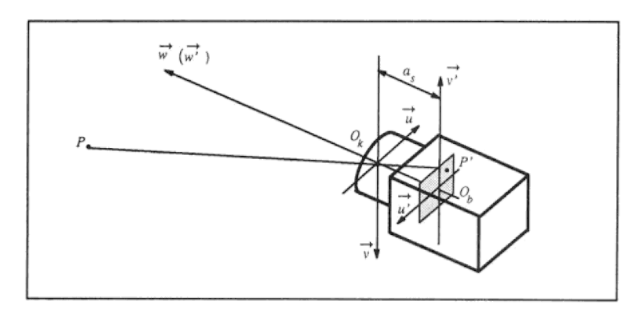
\includegraphics[width=.8\linewidth]{images/kameramodell_vorlaeufig.png}
	\captionof{figure}{Lochkameramodell \cite{Jianzhong}}
	\label{fig:PinholeCamera}
\end{minipage}\\ \\

Koordinatensysteme des Pinhole models erklären: insgesamt werden 5 benötigt um einen 3D punkt auf einen Bildpunkt zu transformieren, mehr dazu im Kapitel \nameref{sec:basisTransformation}

Reconstruction from more than one view:The simplest case is that of two images, which we will consider
first. As a mathematical abstraction, we restrict the discussion to “scenes” consisting of points only.
The usual input to many of the algorithms given in this book is a set of point correspondences.
In the two-view case, therefore, we consider a set of correspondences $x_i \Leftrightarrow x'_i$ in two images.

It is assumed that there exist some camera matrices, $P$ and $P'$ and a set of 3D points $X_i$ that give rise to these image correspondences in the sense that $PX_i = x_i$ and $P'_iX_i = x'_i$. Thus, the point $X_i$ projects to the two given data points. However, neither the cameras (represented by projection matrices $P$ and $P'$), nor the points $X_i$ are known. It is our task to determine them.\\




	Um die Kameramatrix allgemeiner zu formulieren und die Bedeutung und hinter $\zeta$ und dessen Zusammenhang mit dem in der Literatur benutzten $f$ genauer zu erläutern, wird die Kameramatrix der Photogrammetrie in Bezug auf ein Lochkameramodell hier noch einmal genauer betrachtet und mit dem hergeleiteten Modell verglichen\cite{HZ,Heipke}. Zur Beschreibung optischer Kameras greift man üblicherweise auf das Lochkameramodell zurück. Das Modell beruht ausschließlich auf der geometrischen Optik und vernachlässigt physikalische Effekte wie Beugung oder die Auswirkungen der Linse \cite{Heipke}.  Nehmen wir an es gilt $\zeta = f$, dann gilt für die Projektion von Punkten das selbe wie in Gleichung 2.49 nur mit $f$ statt $\zeta$. 

\begin{gather}
\begin{bmatrix}
X\\Y\\Z\\1
\end{bmatrix} \mapsto
\begin{pmatrix}
\zeta X\\ \zeta Y\\ Z
\end{pmatrix}
=
\begin{bmatrix}
\zeta&0&0&0\\
0&\zeta&0&0\\
0&0&1&0
\end{bmatrix}
\cdot
\begin{bmatrix}
X\\Y\\Z\\1
\end{bmatrix}
=
\begin{pmatrix}
\zeta \frac{X}{Z}\\ \zeta \frac{Y}{Z}\\1
\end{pmatrix}\\
\leadsto
\begin{bmatrix}
X\\Y\\Z\\1
\end{bmatrix} \mapsto
\begin{pmatrix}
f X\\ f Y\\ Z
\end{pmatrix}
=
\begin{bmatrix}
f&0&0&0\\
0&f&0&0\\
0&0&1&0
\end{bmatrix}
\cdot
\begin{bmatrix}
X\\Y\\Z\\1
\end{bmatrix}
=
\begin{pmatrix}
f \frac{X}{Z}\\ f \frac{Y}{Z}\\1
\end{pmatrix}
\end{gather}

Zum Vergleich dient die Definition im Buch von \textit{Hartley \& Zisserman}\cite{HZ}, welche der selbst hergeleiteten entspricht.


\begin{gather}
\begin{bmatrix}
X\\Y\\Z\\1
\end{bmatrix} \mapsto
\begin{pmatrix}
f X\\ f Y\\ Z
\end{pmatrix}
=
\begin{bmatrix}
f&0&0&0\\
0&f&0&0\\
0&0&1&0
\end{bmatrix}
\cdot
\begin{bmatrix}
X\\Y\\Z\\1
\end{bmatrix}
\end{gather}		


Die Kameramatrix $K$ lautet in der Literatur\cite{HZ}:

\begin{gather}
K=\begin{bmatrix}
\alpha_x&s&x_{0}\\
0&\alpha_y&y_{0}\\
0&0&1
\end{bmatrix}
\end{gather}

Anstelle von $f$ steht in der Kameramatrix aus Gleichung 2.42 $\alpha_x$ und $\alpha_y$. Die Werte welche $\alpha_x$ und $\alpha_y$ annehmen können, hängen von der geometrischen Form der Pixel des in der Kamera verbauten Sensors ab\cite{HZ,Photonik}.  $\alpha_x$ und $\alpha_y$ sind genau dann einheitlich, wenn die Form der verbauten Pixel, ebenfalls einheitlich quadratisch ist. Die Einheiten der x- und y- Achsen des Sensorkoordinatensystems sind einheitlich. $\alpha_x$ und $\alpha_y$ sind also genau dann ungleich, wenn die auf dem Sensor verbauten Pixel beispielsweise rechteckig oder die geometrische Form eines Parallelogramms besitzen\cite{HZ}. Im Stereoaufbau dieser Arbeit, wurden Kameras mit CMOS-Chips mit quadratischen Pixeln verwendet, weshalb $\alpha_x$ und $\alpha_y$ einheitlich sein werden. $\alpha_x$ und $\alpha_y$ entstehen aus der Multiplikation der Werte für $\zeta_x$ und $\zeta_y$ beziehungsweise  $f_x$ und $f_y$ mit einem jeweiligen Skalierungswert $m_x$ und $m_y$. Sind die Pixel nicht quadratisch, wird auf die Werte $f_x$ und $f_y$ jeweils eine Skalierung $m_x$ und $m_y$ drauf multipliziert so dass  $\alpha_x = f_x \cdot m_x$ und $\alpha_y = f_y \cdot m_y$ entspricht\cite{HZ}. Die Matrixeinträge,$x_{0}$ und $y_{0}$, bilden einen Translationsvektor. Sie beinhalten die Position des Hauptpunkts auf der Bildebene. $x_{0}$ und $y_{0}$ sind definiert als $x_{0} = p_x \cdot m_x$ und $x_{0} = p_y \cdot m_y$. Der Matrixeintrag $s$ wird dem sogenannten \textit{skew-Faktor} zugeordnet, welcher nur dann zum Einsatz kommt, sollte die optische Achse nicht orthogonal auf den Bildsensor auftreffen. Sprich wenn der Chip geneigt in der Kamera montiert wurde\cite{HZ}. Die komplette Projektionsmatrix $P=KR=K[C|v]$ beziehungsweise wie sie in der Literatur zitiert wird $P=K[R|t]$\cite{HZ} besteht aus der Matrixmultiplikation der hergeleiteten Transformationsmatrix $R$ welche die externen Kamerparameter repräsentiert und der Kameramatrix $K$, welche die internen Kameraparameter repräsentiert. $P$ beinhaltet also sowohl die internen als auch die externen Kameraparameter.

\subsection{Kameraparameter}

internen externe parameter\cite{Jianzhong}

Pinhole model. The pinhole model, or perspective projection,
assumes that all camera rays pass through a single point, the optical
center and that there is a linear relationship between image point
position and the direction of the associated camera ray. That relationship
can be expressed via a so-called calibration matrix which depends
on up to five intrinsic parameters:\cite{CamerModels.}\\



Basis Transformationen um Objektpuntke aus sicht der verschiedenen Koordiantensysteme beschreiben zu können \\
Geometrien kurz einführen: benötigte Geometrien sind Homographien, um mit Punkte auf der bildebene zu hantieren \\
Epipolargeometry um geometrische Bezihungen zwischen Bildpunkten, Objektpunkt etx herzustellen